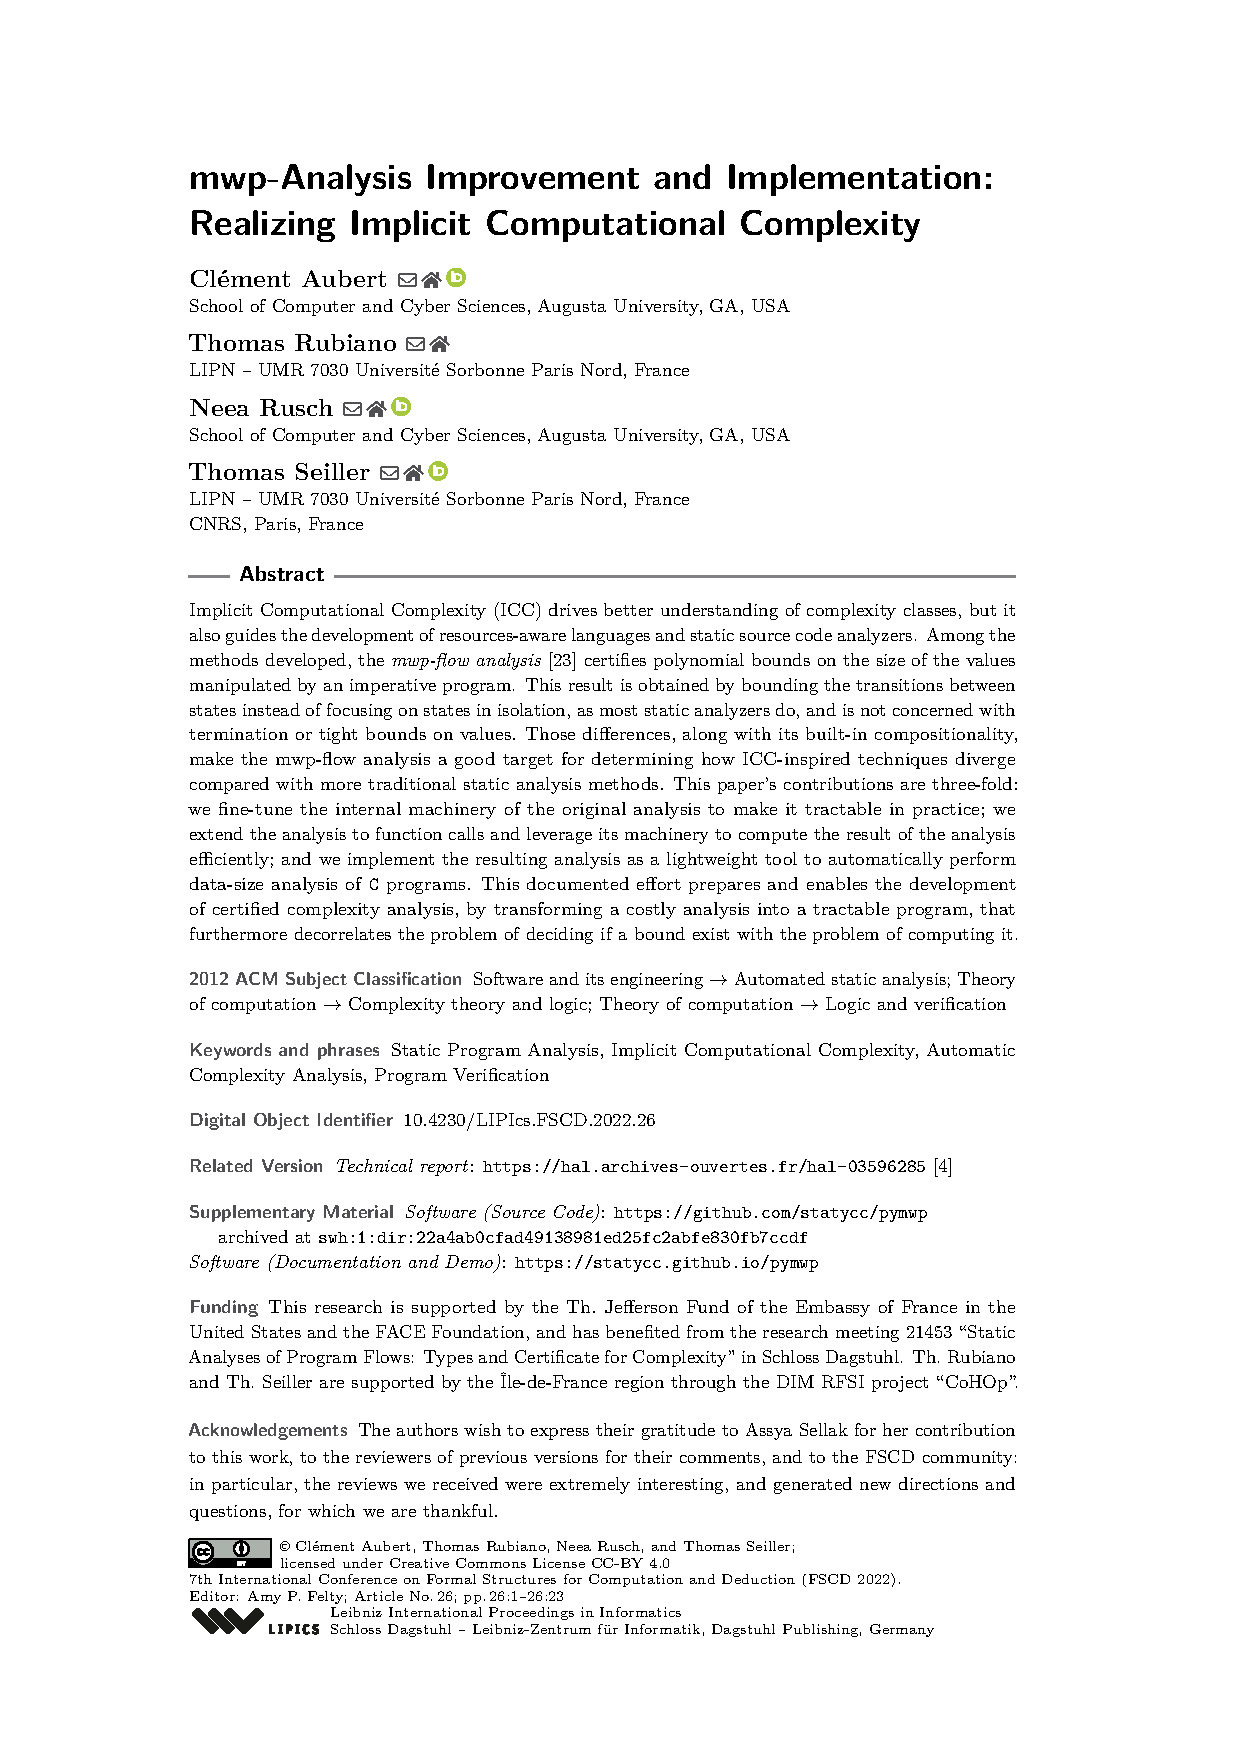
\includepdf[pages={1-},width={\textwidth},frame,offset=0.25in 0in,%
addtotoc={
    2,subsection,2,{Introduction: Letting ICC Drive the Development of Static \mbox{Analyzers}},sec:fscd-intro,
    3,subsection,2,{Background: The Original Flow Analysis},sec:fscd-background,
    3,subsubsection,3,{Language Analyzed: Fragments of Imperative Language},sssec:fscd-lang,
    3,subsubsection,3,{A Flow Calculus of mwp-Bounds for Complexity Analysis},sssec:fscd-calc,
    5,subsubsection,3,{Limitations and Inefficiencies of the mwp Analysis},sssec:fscd-limits,
    6,subsection,2,{A Deterministic, Always-Terminating, Declension of the mwp Analysis},sec:fscd-det,
    7,subsubsection,3,{Internalizing Non-determinism: The Choice Data Flow Semi-rings},sssec:fscd-rings,
    7,subsubsection,3,{Internalizing Failure: De-correlating Derivations and Bounds},sssec:fscd-fail,
    8,subsubsection,3,{Merging the Improvements: Illustrations and Proofs},sssec:fscd-merging,
    10,subsection,2,{Extending and Improving the Analysis: Functions and Efficiency},sec:fscd-extending,
    10,subsubsection,3,{Leveraging Compositionality to Analyze Function Calls},sssec:fscd-comp,
    12,subsubsection,3,{Integrating Recursive Calls, the Easy Way},sssec:fscd-recs,
    13,subsubsection,3,{Taking Advantage of Polynomial Structure to Compute Efficiently},sssec:fscd-poly,
    14,subsubsection,3,{Deciding the Existence of a Bound Faster Thanks to Delta Graphs},sssec:fscd-dg,
    15,subsection,2,{Implementing, Testing and Comparing the Analysis},sec:fscd-eval,
    15,subsubsection,3,{Experimental Evaluation},sssec:fscd-eval,
    15,subsubsection,3,{Related Tools and Incompatible Metrics},sssec:fscd-metrics,
    16,subsection,2,{Conclusion: Limitations, Strengths and Future Work},sec:fscd-conc,
    20,subsection,2,{Appendix A: Technical Appendix on Semi-rings (Abridged)},sec:fscd-app-a,
    21,subsection,2,{Appendix B: Omitted Proofs},sec:fscd-app-b,
    22,subsection,2,{Appendix C: Benchmarks},sec:fscd-app-c,
    22,subsubsection,3,{Descriptions of Program Groups},sssec:fscd-groups,
    22,subsubsection,3,{Results},sssec:fscd-results,
    22,subsubsection,3,{Comparison},sssec:fscd-comparison
}, addtolist={
    4,figure,{Original non-deterministic flow analysis rules},fig-jkrules,
    6,figure,{Deterministic improved flow analysis rules},fig-det-rules,
    23,table,{Benchmark results produced by pymwp on C programs},table:fscd-bench},
    pagecommand={\thispagestyle{plain}%
    \addtoindexm{AProVE}{17}
    \addtoindexm{COSTA}{15}
    \addtoindexm{Cerco}{15}
    \addtoindexm{CoFloCo}{17}
    \addtoindexm{CompCert}{16}
    \addtoindexm{ComplexityParser}{15}
    \addtoindexm{Coq}{16}
    \addtoindexm{Gröbner basis}{13}
    \addtoindexm{Resource Aware ML}{15}
    \addtoindexm{SPEED}{15}
    \addtoindexm{Verasco}{15}
    \addtoindexm{certified-llvm}{16}
    \addtoindexm{complexity classes!\textsc{np}}{6}
    \addtoindexm{complexity classes!\textsc{p}}{3}
    \addtoindexm{delta graph}{14,15}
    \addtoindexm{monomial}{13,14}
    \addtoindexm{mwp-bound}{14,15}
    \addtoindexm{mwp-matrix}{3,5,6,7,8,10,12,13,14,15,20,21,22}
    \addtoindexm{nondeterminism}{4,5,6,7,11,14}
    \addtoindexm{intermediate representation}{6}
    \addtoindexm{pymwp}{15,16,17,22,23}
    \addtoindexm{quasi-invariant}{15}
    \addtoindexm{state explosion}{5,6}
    \addtoindexm{static single assignment}{16}
    \addtosymbolsm{PsiProd}{12}
    \addtosymbolsm{Psi}{12}
    \addtosymbolsm{ai}{7,12,13,14}
    \addtosymbolsm{alpha}{3,4,7,12,13,20}
    \addtosymbolsm{assgn}{7,9,10,11,14,21}
    \addtosymbolsm{beta}{3,4,7,12,13,20}
    \addtosymbolsm{card}{7,14}
    \addtosymbolsm{cartpi}{7,12,13,14}
    \addtosymbolsm{chunk}{11,12}
    \addtosymbolsm{ci}{7,12,13}
    \addtosymbolsm{cj}{7,12,13,14}
    \addtosymbolsm{closure}{3,4,6,11}
    \addtosymbolsm{cmat}{4,6,9,11,21}
    \addtosymbolsm{delta}{7,8,9,10,11,12,13,14,15}
    \addtosymbolsm{f}{10,11}
    \addtosymbolsm{gamma}{3,13}
    \addtosymbolsm{hp}{4}
    \addtosymbolsm{infty}{6,7,8,10,13,14,17,21,22,23}
    \addtosymbolsm{iso}{7,8,20}
    \addtosymbolsm{k}{7,10,12,13,14}
    \addtosymbolsm{map}{6,7,8}
    \addtosymbolsm{matrix}{3,4,6,7,9,10,11,20,21}
    \addtosymbolsm{mi}{3,4,6,7,20}
    \addtosymbolsm{mj}{3,4,6,7,20}
    \addtosymbolsm{msring}{3,7,12,13,21}
    \addtosymbolsm{mstar}{3,4,6}
    \addtosymbolsm{mwpi}{7,9,12,13,14,21}
    \addtosymbolsm{mwpset}{3,6,7,9,13}
    \addtosymbolsm{mzeroj}{4,6}
    \addtosymbolsm{m}{3,4,5,6,7,8,9,11,12,13,20,21}
    \addtosymbolsm{oplus}{3,4,6,8,9,10,11,12,20,21}
    \addtosymbolsm{otimes}{3,4,6,8,11,12,20}
    \addtosymbolsm{plusi}{7}
    \addtosymbolsm{p}{3,4,5,6,7,8,9,11,12,13,20}
    \addtosymbolsm{slot}{11,12,21}
    \addtosymbolsm{smpi}{5,8,9,12}
    \addtosymbolsm{sring}{7,20}
    \addtosymbolsm{timesi}{7,17}
    \addtosymbolsm{v0a}{4,6}
    \addtosymbolsm{vadd}{4,5,8}
    \addtosymbolsm{vare}{4}
    \addtosymbolsm{vec2}{5,7,8,11,12,13,21}
    \addtosymbolsm{vec}{4,8,11}
    \addtosymbolsm{vlist}{4}
    \addtosymbolsm{vrep}{4,6,8,10,12}
    \addtosymbolsm{w}{3,4,5,6,7,8,9,11,12,13,20,21}
    \addtosymbolsm{zero}{3,4,5,6,7,8,9,11,12,13,20}
    }]{pdf/pubs_fscd.2022.pdf}